\documentclass{article}
\usepackage{graphicx}
\usepackage{url}
\title{UI Design Milestone 1}
\author{
    Alex Hart \and Dan Levy \and Mike McGuire
    \and Jessica Perrie \and Corey Young 
}
\date{\today}
\begin{document}
\maketitle

\section{Brainstorming}
Our first step was to decide on the topics needed to be brainstormed. We decided
to look at two users (Rob Smith and Condoleezza Fernandez) from very different
backgrounds, the application's primary functions and the application design.
We used mind-maps to organize our sessions; this allowed for the free forming of
information as it was expressed, imposing few constraints (other than the
specified topic). 

Initially the mind-maps were done by hand on poster paper. They were then
reproduced on a computer for easier updating (if the user needs and software/user
interface are changed) and inclusion in documentation. The user's maps are
detailed in Figures \ref{fig:user1} and \ref{fig:user2}.

\begin{figure}[h!]
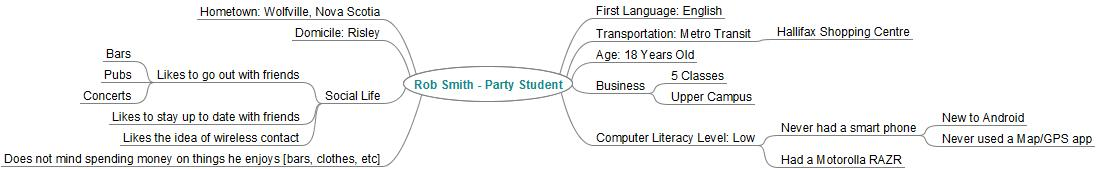
\includegraphics[width=\textwidth]{img/Rob.jpg}
\caption{User 1: Rob Smith}
\label{fig:user1}
\end{figure}

\begin{figure}[h!]
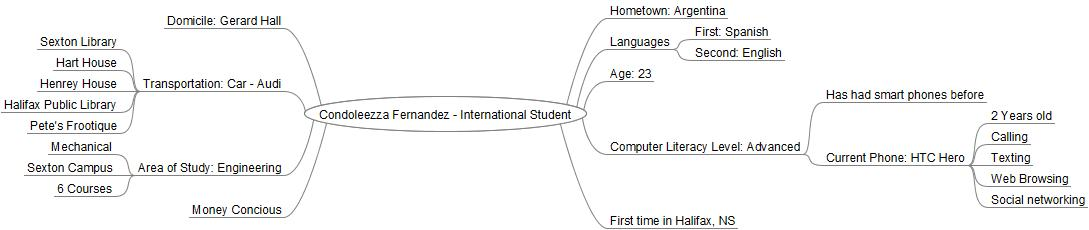
\includegraphics[width=\textwidth]{img/Condoleezza.jpg}
\caption{User 2: Condoleezza Fernandez}
\label{fig:user2}
\end{figure}

When looking at user persona's we decided it would be best to create one at each
end of the computer literacy and/or smart phone experience scale. We looked at
two students; one who was born in Canada, taking Business, not very tech-savvy
and likes to enjoy himself. The other is an international student who is in
Mechanical Engineering, very tech-savvy, money conscious and on the go.

The tasks that we outlined were:
\begin{itemize}
\item Find/browse for a classroom on campus
\item Find the closest wireless hotspot
\item Find my next class with directions from current location
\item Notify the user if they are late for a class, as well as giving directions to
the proper location
\item Create a bookmark of the current location
\item Find a local restaurant (e.g. the closest pizza restaurant)
\end{itemize}

The software's architecture was broken down into two sections: the primary
functions, depicted in Figure \ref{fig:functions}, and an idea for the design of
the software (Figure \ref{fig:design}.

\begin{figure}[h!]
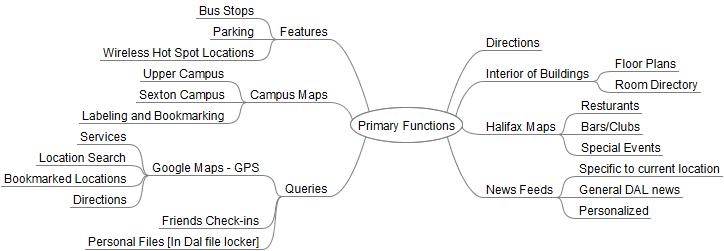
\includegraphics[width=\textwidth]{img/Primary-Functions.jpg}
\caption{The application's primary functions}
\label{fig:functions}
\end{figure}

\begin{figure}[h!]
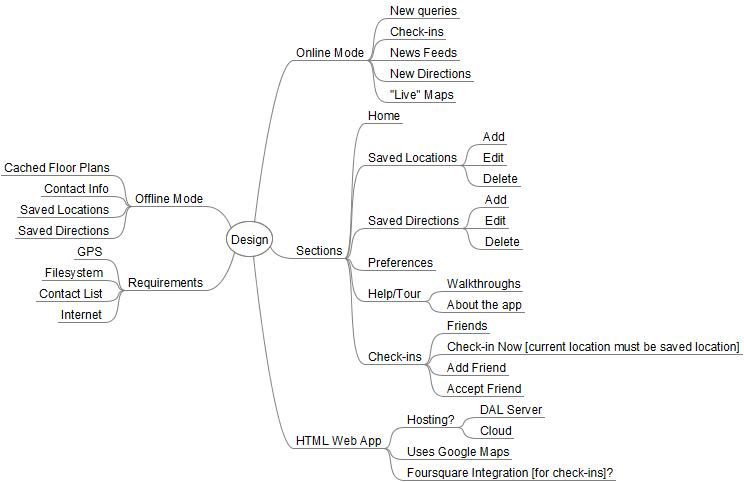
\includegraphics[width=\textwidth]{img/Design.jpg}
\caption{The application's design}
\label{fig:design}
\end{figure}

Our ideas were to either create an Android application, or an web application
(which would allow for use on a higher number of platforms). No matter which
platform we would choose, we planned on using Google services (Maps, Search,
etc) to simplify the application creation. This would allow the application to
meet the primary and secondary functionality requested (showing campus buildings
and services, local information, search, etc). By building a Dalhousie check-in
feature, we give the application a social spin.

In the end we chose to program the proof of concept application in HTML, because
it is platform independent, there is less of a learning curve for the less
experienced programmers in the group and it will be quicker to create.

\section{Use Cases}
\subsection{Meet a Friend}
The user wishes to arrange a place to meet a friend between classes.
The friend has communicated the location of their prior class, and the user
wants to find a meeting place between the friend's class and their own.

To do this, the user opens the Campus Mapper application, and enters the
friend's classroom into the search bar. The application locates the classroom,
and displays a menu with an option to \emph{Show location}. The application
then shows a map centred on the classroom. The user zooms out until their own
classroom is visible (marked by a `Saved location' indicator), and chooses a
suitable meeting place between the two. The user can optionally select the
chosen location and send it to their friend via email or SMS.

\subsection{Closest Wireless Hotspot}
The user wishes to connect to the university's wireless network. They would like
to know the location of the nearest wireless hotspot.

The user opens the Campus Mapper application, and hits the Menu button. The
application displays a menu containing a \emph{Find wireless} option.
The user selects \emph{Find wireless}. The application locates the nearest
university wireless hotspot, and presents a menu containing options to
\emph{Show location}, and to \emph{Get directions}. The user may select either
option; \emph{Show location} will show a map centred on the hotspot, \emph{Get
directions} will provide walking directions from the user's location to the
hotspot.

\subsection{Find a Classroom on Campus}
The user wishes to locate a classroom on campus. Currently, the user must either:
\begin{itemize}
\item Look up classroom information on Dal's website.  User is given street
address, building name, and classroom number. 
\item Phone a friend to ask for directions (e.g ``Beside Building A, go
downstairs, can't miss it'')
\item Type the address into Google maps. The user is given a visual
representation of the building's location, but no directions as to where exactly
the room is located. 
\end{itemize}

With the Campus Mapper application, they would follow these steps:
\begin{enumerate}
\item User opens the CampusMapper application on their smartphone. 
\item The user can then either:
    \begin{itemize}
    \item The user can choose to use the search function (`room 242 LSC'), then
    choose the classroom from the given results, or
    \item The user can open the \emph{Find Classroom} function, select `LSC' under
    buildings, then select `Room 242' from a given drop-down menu.
    \end{itemize}
\item The user will be given a map that displays the users given location (based on
GPS coordinates) and a direct path to the entrance of the building (much like
Google maps).
\item Once the user arrives at the building, there will be a second set of
directions given to the user, that describe how to get to the classroom from the
entrance of the building, (e.g. Take the elevator to floor 2. After exiting the
elevator, turn right. Room 242 is at the end of the hallway on your left).
\item Optionally, the user can now save this path by selecting `Save Path' which
adds it to the user's bookmarks.
\end{enumerate}

\subsection{Notification of Tardiness}
The user is in the library studying for a test and loses track of time. Without
the Campus Mapper application, the user might get a text from a friend, asking
``Why aren't you in class?'', or perhaps the user's alarm notifies them that they
are late. It is possible that the user can't remember the current days schedule.

If the user had the Campus Mapper application:
\begin{itemize}
\item The user receives a notification from the Campus Mapper app that they have
a class beginning in 15 minutes.
\item The user chooses from a set of presented options:
    \begin{description}
    \item[Ignore] - Will close the notification. The user will not be reminded
    about it again. 
    \item[Remind me later] - Reminds the user again (in five minutes).
    \item[Directions] - `Show me how to get there'. Takes the user to the \emph{Get
    Directions} feature, pre-configured with the building and classroom info for
    the class.
    \end{description}
\end{itemize}

\subsection{Create a Bookmark}
When the user finds a location that they want the system to remember, they can
bookmark it. This will add this location to a `Bookmarks' list, which will be
accessible in the other functions of the Campus Mapper application, for
instance:

\begin{itemize}
\item The user can select the location from the bookmarks list, and have the
location automatically pointed out to them on the map.
\item The bookmark will also allow the user to be directed to the building via
the \emph{Get Directions} feature.
\end{itemize}

\subsection{Find a Local Restaurant}
Restaurants are marked on the Campus Mapper map. The user can interact with
these locations to:
\begin{itemize}
\item Learn more information about them. This information could include reviews,
hours of operation, street address, etc.
\item Get directions to them. This functionality would use their current GPS
location, if one is available.
\end{itemize}
In addition, when a user arrives at a recognized location, they can (optionally)
be `signed in' to the location on Foursquare.

\section{Personas}
\subsection{Rob Smith}
\begin{tabular}{ll}
Age: & 18 \\
Field of Study: & Management \\
Residence: & Risley Hall \\
\end{tabular}

\subsubsection{User Background}
Rob Smith is an 18 year old English speaking Management student entering his
first year of University. With a course load of only 4 classes, he plans on
having ample spare time for enjoying the Halifax night life while studying. He
is originally from Wolfville, NS, and has limited knowledge of the campus and
surrounding area, since he has only visited the city during his summer vacations
as a high school student. Rob would describe himself as an inexperienced
computer-user, without a history of Smartphone use. His current cellular device
is a Motorola Razer and is used primarily for making phone calls and
sending/receiving occasional text messages.  He does not own a vehicle, making
the bus his primary mode of transportation.

Areas of campus most often used by this user:
\begin{itemize}
\item Killam Library
\item Student Union Building 
\item Rowe Building
\item Dalplex 
\end{itemize}

Off campus:
\begin{itemize}
\item The Palace Nightclub
\item Pizza Corner 
\end{itemize}

\subsection{Condoleezza Fernandez}
\begin{tabular}{ll}
Age: & 23 \\
Field of Study: & Mechanical Engineering \\
Residence: & Gerard Hall \\
\end{tabular}

\subsubsection{User Background}
Condoleezza Fernandez is a 23 year old Mechanical Engineering student,
originally from Argentina. Her first language is Spanish but has learned enough
English from home to consider herself bi-lingual. She has recently arrived in
Halifax, and is not yet familiar with the Studley or Sexton campuses. Being the
owner of a vehicle, she intends to get to know Halifax as well as the
surrounding Areas of Dartmouth and Bedford.  Condoleezza considers herself to be
an advanced computer user, keeping up to date with the latest trends in
technology. Her current cellular device is an Android (HTC Hero) which she has
owned for two years.  She uses her Smartphone for calling, texting, web browsing
and updating her social network profiles. 

Areas of campus most often used by this user:
\begin{itemize}
\item Sexton Library (A, B, C Building) 
\item Hart House 
\item Henry House
\end{itemize}

Off campus:
\begin{itemize}
\item Halifax Public Library
\item Pete’s Frootique
\end{itemize}

% ==============================================================================
\section{Narratives}
\subsection{Rob Smith}
\subsubsection{Scenario to Find Buildings and Services (Currently)}

Rob is not from Halifax, he grew up in the Annapolis Valley. Rob has visited
Halifax before moving there to shop, go to the concerts, and go out to dinner.
He is farmiliar with the different parts of the city (Dartmouth, Halifax,
Burnside, etc), but not with any great detail. when visiting Rob would have his
city map ready, as well as pre-decided routes to the locations he wanted to go.

When Rob is looking for a class or building on campus he usually takes two
routes; asking a friend or classmate or going to an on campus computer to try
and look up directions. When looking for an on campus location or event online
sometimes he needs to visit a few different sites depending on what he is
looking for --- Google Maps, Dalhousies' various online maps, the coast website,
etc. 

When Rob needs an on campus service he will usually check the Dalhousie website
or ask people who may know on campus.

\subsubsection{Scenario to Find Buildings and Services (Future with App)}
With the application Rob now is able to go to one location to find buildings on
campus, and local businesses. He can look at the Dalhousie directory to find
information about when offices are open and the search function to find
direction offices, or local establishments. With the check-in feature Rob can
see where his friends are.

Rob does not need to worry about being late for class as it knows his schedule
(DalOnline integration) and class locations; prompting him when he is not in the
proper location during each class (using GPS to determine this information).

Rob can also bookmark his favorite locations, this way he can get directions to
them from anywhere he may be, giving him driving, walking or public transit
directions.

\subsection{Condoleezza Fernandez}
\subsubsection{What They Do Now (To Find Buildings and Services)}

Condoleezza is afraid of getting lost and missing time to study. Hence, to find
buildings or services on campus, she usually references multiple online maps,
such as the Campus Map (currently in Beta), a Sexton Campus Map and directions
from people or online sources before going to the locations.

For buildings on campus, she first checks the online Sexton Campus Map as
suggested by one of her older engineering friends who used the map when he
started at Dalhousie. However, because the Sexton Map doesn’t show her where the
Henry House is located, she decides to check the online Campus Map linked from the
Dalhousie site. On the Campus Map she searches for the house, but it doesn’t
appear in her results. Although she is confused, she trusts the Campus Map because
it let her know that the house is not included in its locations, and she plans
to ask her friends if “Henry House” is spelled correctly. On the Campus Map, she
finds other buildings and memorises the buildings’ appearance and surroundings.

To locate services on campus, she first checks the Sexton Campus Map.
Remembering that it was not complete in showing her the Henry House, she also
checks the Campus Map and memorises where the services are located.

On arriving closer to the buildings or services, she asks friends or complete
random strangers for directions. Sometimes their directions are not clear;
however, they confirm her location and increase her trust for the online maps.
On approaching her destination, she also looks for physical signs and other maps
or landmarks.

\subsubsection{Scenario to Find Buildings and Services (Future with App)}

Because Condoleezza is able to contact her friends while using the App, it is
more frequently used by her friends. Hence, they suggest that she use it for all
her building and service searches. She searches for buildings on campus using
the App and saves their locations to her favourites. If a building is not found,
she immediately contacts her friends to ask for the correct name or location of
the building. 

To find services on campus, she searches for them on the App. She chooses
certain services around her most frequented locations and saves them to her
favourites. When she goes around campus, using her smart phone and the App, she
follow the directions and floor plans to her favourite locations; thus, she
relies less on other peoples’ directions.

\subsubsection{Links}
\begin{itemize}
\item Campus Map Beta \hfill                      \url{http://campusmap.dal.ca/}
\item Sexton Campus Map \\
                      \hfill \url{http://fm.dal.ca/campusmap/index.php?campus=X}
\end{itemize}
\end{document}
